\documentclass[zihao=false,fontset=windows]{ctexart}
% ctexart 不接受任意 pt 选项。正文改 {10pt}，方括号里是行距。
\usepackage{scrextend}
\changefontsizes[12pt]{10pt}

\usepackage[a4paper,left=2.35cm,right=2.35cm,top=1.7cm,bottom=1.9cm]{geometry}
\usepackage{xcolor}
\usepackage{graphicx}
\usepackage{amsmath,amssymb}
\usepackage{enumitem}
\usepackage{tabularx}
\usepackage{colortbl}
\usepackage{listings}
\usepackage{hyperref}
\usepackage[most]{tcolorbox}
\usepackage{textcomp}

\definecolor{feishuText}{RGB}{31,35,41}
\definecolor{feishuBlue}{RGB}{36,91,219}
\definecolor{feishuRed}{RGB}{216,57,49}
\definecolor{feishuGreen}{RGB}{46,161,33}
\definecolor{feishuGray}{RGB}{100,106,115}
\definecolor{feishuGray2}{RGB}{143,149,158}
\definecolor{feishuPinkBg}{RGB}{251,191,188}
\definecolor{quoteBar}{RGB}{51,112,255}
\definecolor{codebg}{RGB}{245,246,247}
\definecolor{codeborder}{RGB}{222,224,227}
\definecolor{inlinebg}{RGB}{242,243,245}
\definecolor{callRed}{RGB}{253,226,226}
\definecolor{callOrange}{RGB}{255,245,235}
\definecolor{callYellow}{RGB}{254,255,240}
\definecolor{callGreen}{RGB}{240,251,239}
\definecolor{callBlue}{RGB}{240,244,255}
\definecolor{callRedSoft}{RGB}{254,241,241}
\definecolor{callSun}{RGB}{255,255,204}
\definecolor{callGreenPage}{RGB}{217,245,214}
\definecolor{callOrangePage}{RGB}{254,234,210}
\definecolor{hlYellow}{RGB}{255,246,122}
\definecolor{tableHead}{RGB}{242,243,245}
\definecolor{tableRule}{RGB}{222,224,227}
\definecolor{codeText}{RGB}{31,35,41}
\definecolor{codeKeyword}{RGB}{0,0,255}
\definecolor{codeComment}{RGB}{0,128,0}
\definecolor{codeString}{RGB}{163,21,21}

\setmainfont{Times New Roman}
\setCJKmainfont{Microsoft YaHei}[AutoFakeBold=2.2]
\setCJKsansfont{Microsoft YaHei}[AutoFakeBold=2.2]
\setCJKmonofont{Microsoft YaHei}[AutoFakeBold=2.2]
\setmonofont{Consolas}
\newfontfamily\emojifont{Segoe UI Emoji}

\hypersetup{
  colorlinks=true,
  urlcolor=feishuBlue,
  linkcolor=feishuBlue,
  unicode=true,
  pdftitle={BLIP(2022, Salesforce)}
}

\setlength{\parindent}{0pt}
\setlength{\parskip}{0.42em}
\setlength{\fboxsep}{1.5pt}
\setlength{\emergencystretch}{3em}
\linespread{1.28}
\color{feishuText}
\arrayrulecolor{tableRule}
\urlstyle{same}

\setlist[enumerate]{label=\textcolor{feishuBlue}{\arabic*.}, leftmargin=1.7em, itemsep=0.22em, topsep=0.28em, parsep=0.08em, partopsep=0pt}
\setlist[itemize,1]{label=\textcolor{feishuBlue}{\textbullet}, leftmargin=1.35em, itemsep=0.18em, topsep=0.25em, parsep=0.06em, partopsep=0pt}
\setlist[itemize,2]{label=\textcolor{feishuBlue}{◦}, leftmargin=1.45em, itemsep=0.12em, topsep=0.15em}
\setlist[itemize,3]{label=\textcolor{feishuBlue}{\rule[0.18em]{0.38em}{0.38em}}, leftmargin=1.55em, itemsep=0.1em, topsep=0.12em}

\newcommand{\feiEmoji}[1]{{\emojifont #1}}
\newcommand{\incode}[1]{\colorbox{inlinebg}{\ttfamily\small #1}}
\newcommand{\bigmath}[1]{%
  \begin{center}\large$\displaystyle #1$\end{center}%
}
\newcommand{\hy}[1]{\colorbox{hlYellow}{\textbf{#1}}}
\newcommand{\hp}[1]{\colorbox{feishuPinkBg}{\textbf{#1}}}

\lstset{
  language=Python,
  basicstyle=\ttfamily\footnotesize\color{codeText},
  keywordstyle=\color{codeKeyword},
  commentstyle=\color{codeComment},
  stringstyle=\color{codeString},
  showstringspaces=false,
  breaklines=true,
  columns=fullflexible,
  keepspaces=true,
  tabsize=4,
  upquote=true,
  aboveskip=2pt,
  belowskip=0pt,
  xleftmargin=0pt,
  frame=none
}

\tcbset{
  feishubase/.style 2 args={
    enhanced,
    boxrule=0pt,
    arc=8pt,
    left=10pt,
    right=10pt,
    top=7pt,
    bottom=7pt,
    before skip=6pt,
    after skip=6pt,
    colback=#1,
    colframe=#1,
    before upper={\feiEmoji{#2}\hspace{0.45em}\ignorespaces}
  }
}
\newtcolorbox{feishubox}[2]{feishubase={#1}{#2}, breakable}
\newtcolorbox{feishuboxnb}[2]{feishubase={#1}{#2}}

\newtcolorbox{feishuquote}{
  enhanced,
  breakable,
  boxrule=0pt,
  leftrule=3pt,
  arc=0pt,
  colframe=quoteBar,
  colback=white,
  left=8pt,
  right=2pt,
  top=2pt,
  bottom=2pt,
  before skip=4pt,
  after skip=4pt,
  before upper=\color{feishuGray}
}

\newtcolorbox{feishucode}{
  enhanced,
  breakable,
  colback=codebg,
  colframe=codeborder,
  boxrule=0.6pt,
  arc=6pt,
  left=6pt,
  right=6pt,
  top=5pt,
  bottom=4pt,
  before skip=6pt,
  after skip=6pt
}

\begin{document}
{\zihao{1}\bfseries BLIP(2022, Salesforce)\par}

\begin{feishuquote}
BLIP：既能理解又能生成（2022，Salesforce）\par
\href{https://arxiv.org/abs/2201.12086}{Bootstrapping Language-Image Pre-training}\par
\end{feishuquote}

在 ALBEF 之后，作者团队又于 2022 年在 ICML 上发表了后续工作：BLIP。BLIP 基本上可以看做是吸收了 VLMo 思想的 ALBEF，它的训练目标和技巧基本都与 ALBEF 一致。\par

\par\vspace{1.15em}\noindent{\zihao{-2}\bfseries 1. 概述}\par\vspace{0.28em}
BLIP既可以做内容理解，还可以做文本生成，是一个大一统的多模态预训练框架，并且提出了通过引导 caption 来去除噪声的方法。（\textcolor{feishuRed}{\textbf{理解+生成 }}）\par
BLIP在各个下游任务上展现出了强大的性能，并且具有 zero-shot 的能力。\par

{\renewcommand{\arraystretch}{1.35}%
\begin{tabularx}{\textwidth}{|>{\raggedright\arraybackslash}X|>{\raggedright\arraybackslash}X|}
\hline
\cellcolor{callOrange}动机 & \cellcolor{callYellow}改进方法 \\
\hline
\hy{模型角度}：VLP大多采用了Encoder-only 模型或者Encoder-Decoder模型。但是Encoder-only 模型 \textbf{很难实现文本生成}，并且Encoder-Decoder 模型\textbf{不能直接用于多模态检索或理解型任务}。
&
\hp{多模态编码器-解码器混合结构（MED）}：一种用于有效的多任务训练和灵活迁移学习的新框架。包含\textbf{单模态编码器}、\textbf{基于图像的文本编码器}、\textbf{基于图像的文本解码器}。用三个损失进行预训练：图文对比损失（ITC）、图文匹配损失（ITM）、图像条件语言建模（LM）。 \\
\hline
\hy{数据角度}：无论是CLIP、ALBEF训练的image-text 都是从web收集的，其中包含很多\textbf{noisy data}，vision-language训练是次优解
&
\hp{Captioning and Filtering（CapFilt）}：一种从噪声图文对中学习的新的数据增强方法。预训练的 MED 分为两个模块：Captioner 模块用于给 web 图像生成对应文本；Filter 模块用于从原始的 web 文本和生成的文本中剔除噪声。 \\
\hline
\end{tabularx}}

\begin{feishuquote}
BLIP本质上还是想做图文配对的自然语言理解任务的，但是为了处理数据，优化网上的数据集配对情况，不得已搞出了生成任务，以此优化图片配对情况，从而进行更好的训练。\par
\end{feishuquote}

\begin{feishubox}{callGreenPage}{🙋}
Encoder-Decoder 模型不能用于检索或是理解的原因：\par
\textcolor{feishuBlue}{Encoder-Decoder模型是一种生成式模型，主要用于机器翻译和文本摘要等任务。在多模态检索任务中，需要从图像中提取特征，并与文本特征进行匹配，以实现图像和文本的关联。而Encoder-Decoder模型并没有设计用于从图像中提取特征，也没有考虑如何处理图像和文本之间的语义鸿沟，因此不能直接用于多模态检索任务。}\par
\end{feishubox}

\par\vspace{1.15em}\noindent{\zihao{-2}\bfseries 2. 模型结构}\par\vspace{0.28em}
\begin{center}
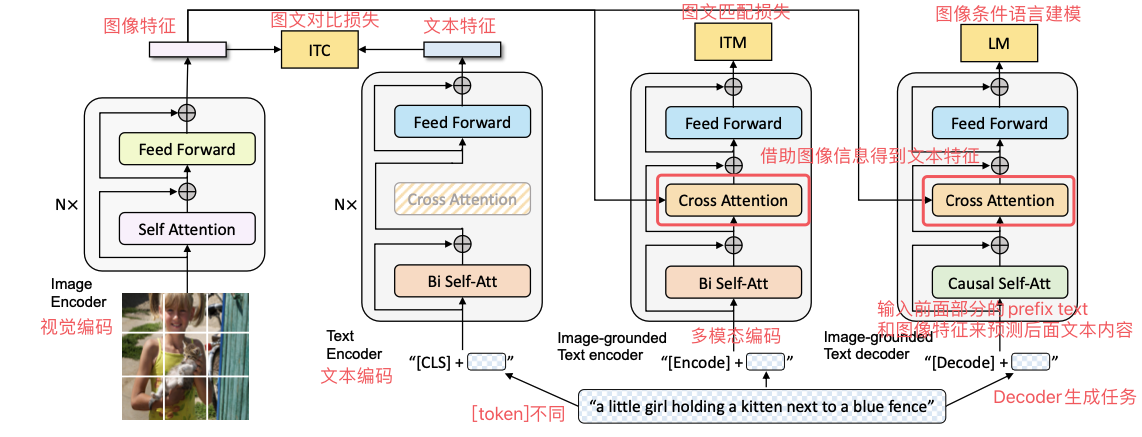
\includegraphics[width=0.98\textwidth]{images/2022-ICML-BLIP/fig-01.png}
\end{center}
BLIP 提出了\textbf{多模态混合（multimodal mixture of encoder-decoder，MED）}的模型架构，其实就是在 ALBEF 的基础上引入了 decoder 专门去做生成式语言的任务。\par
\begin{feishuquote}
图中左边三列其实就是\href{https://scnajei2ds6y.feishu.cn/wiki/U5sZwCwKwivERwktFWvcdM50nkf}{ALBEF}的结构，可以去对比一下。\par
\end{feishuquote}
它总共分为3个板块，两个encoder和一个decoder：\textbf{Unimodal encoder（image encoder + text encoder）、Image-grounded text encoder、Image-grounded text decoder}：\par
\begin{itemize}
\item \textbf{Unimodal encoder}：
\begin{itemize}
\item \textbf{image encoder }
\begin{itemize}
\item 目的：提取图像特征，\textcolor{feishuBlue}{相当于 CLIP 中的 Image Encoder}
\item ViT架构：将输入图像切分成patches并编码成image embeddings，使用[cls]token来表示全局图像特征。
\end{itemize}
\item \textbf{text encoder }
\begin{itemize}
\item 目的：提取文本特征，\textcolor{feishuBlue}{相当于 CLIP 中的 Text Encoder}
\item BERT架构（\textbf{双向自注意力机制 Bi Self-Att }+ FFN）：输入是[cls]+文本，[cls]token表示整个句子。
\end{itemize}
\item 然后再将图像 embedding 和 文本 embedding 做图文的对比学习 ITC
\end{itemize}
\item \textbf{Image-grounded text encoder 基于图像的文本编码器}：
\begin{itemize}
\item 目的：用来提取文本特征并将其和图像特征对齐，\textcolor{feishuBlue}{相当于 CLIP 中更精细化的 image-text 对齐}
\item 输入是[Encode]+文本。然后分别经过双向 Self-Attention（使得text全部可见） -> \textbf{Cross Attention}（图像的 embedding 会注入到 Cross Attention中进行多模态的学习） -> FFN 后得到输出，得到的 Embedding 和图像的 embedding 做图文匹配任务 ITM。
\item 相比于单模态的文本编码器只多了Cross Attention，他们的双向attention和FFN是共享参数的。
\item 输入时增加了特定的[Encode]token，在输出中[Encode]代表图像文本的联合表征。
\end{itemize}
\item \textbf{Image-grounded text decoder 基于图像的文本解码器}：
\begin{itemize}
\item 目的：用来生成符合图像和文本特征的文本描述，\textcolor{feishuBlue}{这是 CLIP 中所没有的}
\item 输入是[Decode]+文本。使用cross attention，将图像embedding和prefix text（前部分文本）做文本生成的任务，预测下一个token。特定[Decode]token表示序列解码的开始符号，还有一个[EOS] token用于表示序列的结束。
\item 它和基于图像的编码器不同的是：使用的是\textbf{ Causal Attention}，而不是双向的。\par
因为对于 Decoder 而言，它不能看到完整的句子，它要做的事是给定前半句生成后半句，所以要用 Causal Attention，即将后半句给 mask 掉，使得text只能见到当前和历史的文本。（类似于GPT系列）
\item 除了第一层 Causal Attention 外，其它两层和 Image-grounded text encoder 的\textbf{参数是共享}的，所以虽然Decoder新添加了一个 Decoder，但实际上参数量并没有增加很多。
\item 最后的目标函数就是用的 GPT 系列的 Language Modeling（LM），也就是给定一些词，去预测剩下的那些词。
\end{itemize}
\end{itemize}

\begin{feishubox}{callOrangePage}{⚠}
\begin{enumerate}
\item \textbf{图中相同颜色的部分是参数共享的，可以减少很多计算量}。
\item 每个 image-text 对在输入时，\textbf{image 部分只需要过1个图像模型，text 部分需要过3次文本模型}（前两个是encoder，后面是1个decoder）。\par
即 在每一次训练迭代时，图像端只需要做一次forward，但文本端在要做三次forward，要分别通过这三个模型去得到对应的特征，然后去算对应的目标函数，所以\textcolor{feishuBlue}{非常耗时}。
\item Image-grounded text decoder 生成的文本描述不同于输入的image-text对中的文本，image-text对中的文本是web上找到的图片的上下文，拥有大量的噪音；而 Image-grounded text decoder 生成的文本描述是针对图像特征和文本特征的特定描述，更加精炼。这里其实就已经是 Captioner 的雏形了，下面的 Captioner 也是基于训练完成的 Image-grounded text decoder 再进行的优化和微调。
\end{enumerate}
\end{feishubox}

\begin{feishuquote}
\textbf{Causal Attention}：\par
标准的self-attention允许模型关注输入序列中的任何位置，无论这些位置是在当前位置之前还是之后。这意味着模型在处理一个词时，可以看到并基于序列中的所有词进行决策。然而，在某些情况下，让模型看到未来的信息可能会导致问题，例如在序列生成任务中（如机器翻译或文本摘要），如果模型看到了未来的信息，它可能会提前泄露未来的内容，导致生成的文本不连贯或包含未出现的信息。\par
为了解决这个问题，causal attention 被引入。在这种机制中，模型在处理每个位置时只能看到该位置之前的所有信息。这确保了模型不会提前知道未来的内容，从而避免了上述问题。在实践中，causal attention 通常通过为自注意力权重添加一个额外的位置依赖的掩码来实现，该掩码阻止模型看到未来的位置。\par
总结：causal attention是一种特殊的自注意力实现方式，通过限制模型只能看到当前和历史的文本，确保模型不会提前知道未来的内容，从而在一些序列生成任务中提高模型的性能和输出的质量。\par
\end{feishuquote}

\par\vspace{1.15em}\noindent{\zihao{-2}\bfseries 3. 预训练}\par\vspace{0.28em}
BLIP 在预训练期间联合优化了3个目标，两个是理解式任务的loss ，一个是生成式任务的loss。分别是\textbf{Image-Text Contrastive Loss (ITC) }、\textbf{Image-Text Matching Loss (ITM)}、\textbf{Language Modeling Loss (LM)}。\par
BLIP中将ALBEF中的MLM替换成了语言模型（LM）任务，其他与ALBEF保持一致。\par
\begin{enumerate}
\item \href{https://scnajei2ds6y.feishu.cn/wiki/U5sZwCwKwivERwktFWvcdM50nkf\#HFfNdb3hbobohJxMPu3cEHuPnue}{\textbf{ITC}}
\begin{itemize}
\item 作用于image encoder和text encoder。
\item 针对图像编码器和文本编码器，通过正负图文对的对比学习，来对齐图像和文本的潜在特征空间。
\end{itemize}
\item \href{https://scnajei2ds6y.feishu.cn/wiki/U5sZwCwKwivERwktFWvcdM50nkf\#S7ObdE0VwojSbQxDqNJcmZmQnpb}{\textbf{ITM}}
\begin{itemize}
\item 作用于image encoder和image-grounded text encoder。
\item 针对以图像为基础的文本编码器，通过对图文匹配性进行二分类，建模图文多模态信息的相关性。
\item \feiEmoji{⚠} 在ALBEF中，作者的思路是将BERT截成两段，前半段用来做encoder，后半段用来做模态融合。在BLIP这篇工作中，作者分别使用了\textbf{两个完整的BERT结构}分别做encoder和模态交互，同时，这两个BERT结构的self attention和FFN 层的参数是共享的。ITC任务的训练也帮助了ITM任务的训练。
\end{itemize}
\item \textbf{Language Modeling Loss (LM)}
\begin{itemize}
\item 作用于image encoder和image-grounded text Decoder。
\item LM对给定图像生成文本描述。针对以图像为基础的文本解码器，通过交叉熵损失进行优化，训练模型以\textbf{自回归}的方式生成目标caption。在计算损失时，应用了0.1的标签平滑。
\item 与广泛应用于VLP的MLM损失相比，LM使模型具有将视觉信息转化为连贯字幕的泛化能力。其实MLM->LM，就是从BERT->GPT形式（BERT系语言模型几乎都是在MLM任务上做预训练的，GPT系语言模型都是在LM任务上做预训练的）。
\item LM任务会比MLM任务更难，LM任务也更适合生成式的下游任务。
\end{itemize}
\end{enumerate}

\begin{feishubox}{callOrangePage}{⚠}
BLIP是ALBEF的原班人马做的，所以用到了很多ALBEF的技巧:\par
\begin{enumerate}
\item ITC的时候也用了\href{https://scnajei2ds6y.feishu.cn/wiki/U5sZwCwKwivERwktFWvcdM50nkf\#R1iddqHblo2VKPxEzF4cdzAmnIc}{\textbf{Momentum Encoder}}去做更好的Knowledge Distillation和更好的数据级清理。
\item ITM的时候，也像ALBEF一样利用ITC算的Similarity Score做\href{https://scnajei2ds6y.feishu.cn/wiki/U5sZwCwKwivERwktFWvcdM50nkf\#S7ObdE0VwojSbQxDqNJcmZmQnpb}{\textbf{Hard Negative Mining}}，从而每次都用最难的负样本去算ITM，增加Loss的有效性。
\end{enumerate}
\end{feishubox}

以上就是MED的混合形式，它的任务几乎是没变的，ITC、ITM，无非就是把 BERT 的 MLM 任务换成 LM 任务。这就解决了无法做生成任务和理解任务的问题，这样 BLIP 就能把生成和理解统一到一个框架中。\par

\par\vspace{1.15em}\noindent{\zihao{-2}\bfseries 4. "B"->Bootstrapping：CapFilt}\par\vspace{0.28em}
CapFilt提出的动机：\par
\begin{itemize}
\item CLIP还有ALBEF等等虽然爬了4亿的数据进行模型训练，但是从网上搜集到的图文对$(I_w, T_w)$含有噪音，噪音文本无法精确的描述图像的视觉内容，未经清洗和修正可能导致模型训练准确性不高。
\item 高质量的人工注释图像-文本对$(I_h, T_h)$，比如COCO数据集，因为成本高昂所以数量不多。
\end{itemize}
所以，BLIP提出一种高效率利用噪声网络数据的方法\textcolor{feishuRed}{\textbf{Captioning and Filtering (CapFilt)}}，提升图文对的质量。CapFilt包含两个模块：\par
\begin{enumerate}
\item 一个用于给web图像生成字幕（caption）的captioner，增加新的好的文本信息；
\item 一个用于去除噪声图文对的filter，清理、删除不好的、不匹配的文本信息。
\end{enumerate}
captioner和filter都是从相同的预训练 MED 模型初始化的，并在COCO数据集上分别进行微调。调优是一个轻量级的过程。\par
\begin{center}
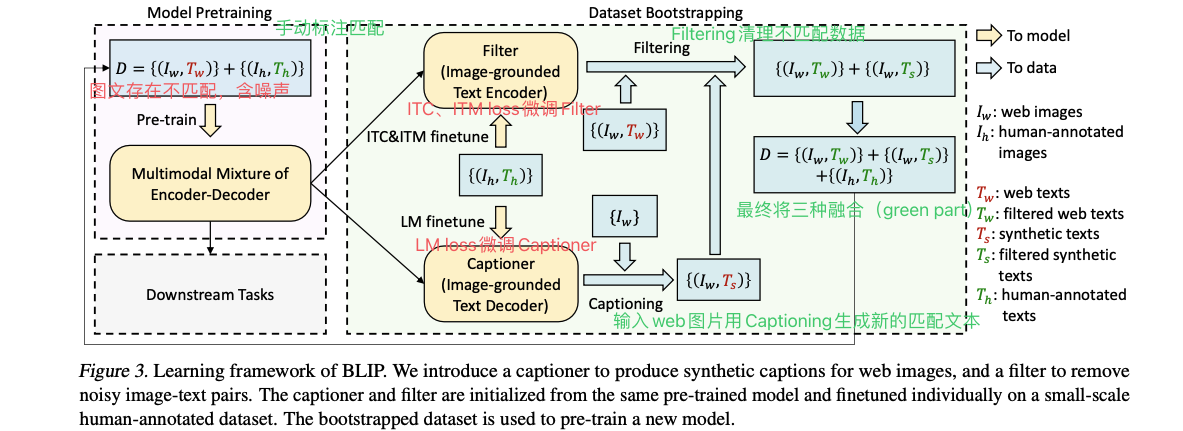
\includegraphics[width=0.98\textwidth]{images/2022-ICML-BLIP/fig-02.png}
\end{center}

\begin{tcbraster}[raster columns=2, raster equal height=rows, raster column skip=9pt, raster row skip=8pt, raster left skip=0pt, raster right skip=0pt]
\begin{feishuboxnb}{callSun}{🌟}
\textcolor{feishuRed}{\textbf{采样生成器captioner}}：\par
Image-grounded Text Decoder基于图像的文本解码器（生成），用LM loss进行微调\par
\end{feishuboxnb}
\begin{feishuboxnb}{callSun}{🌟}
\textcolor{feishuRed}{\textbf{噪声过滤器filter}}：Image-grounded Text Encoder基于图像的文本编码器（判别），用ITC+ITM loss进行微调，判断图文是否匹配，过滤掉噪声图文对\par
\end{feishuboxnb}
\end{tcbraster}

详细过程解释：\par
\begin{itemize}
\item 左侧的 Model Pretraining 就是 MED，训练数据包含了从网上爬的图文对$(I_w, T_w)$和人工标注的图文对$(I_h, T_h)$（人工标注的数据的质量比较好）
\begin{feishuquote}
图中\textcolor{feishuRed}{红色}的$(I_w, T_w)$可以认为包含噪音，\textcolor{feishuGreen}{绿色}的$(I_h, T_h)$可以认为是质量比较好的数据\par
\end{feishuquote}
数据会输入到 MED 当中进行预训练，以 ITC 和 ITM 为目标微调 Image-grounded Text \textbf{Encoder}，以 LM 为目标微调 Image-grounded Text\textbf{ Decoder}。
\item 微调之后，对于网上的任意一个图片$I_w$输入进来，都可以经过（在COCO数据集上经过LM微调的） \textbf{Image-grounded Text Decoder} 来生成\textcolor{feishuRed}{\textbf{字幕}} \textcolor{feishuRed}{\textbf{caption}}，即\textcolor{feishuRed}{红色}的$T_s$。
\item 同时对于 \textcolor{feishuRed}{\textbf{filter}} 来说，在COCO数据集上使用 ITC 和 ITM 微调的 \textbf{Image-grounded Text Encoder}，所以它对图文对的匹配程度的判断是精准的，用它判断生成的 captain 和图片是否匹配，即判断$(I_w, T_s)$是否匹配。同时还可以判断网上爬取的文本对是否匹配，即$(I_w, T_w)$。\par
如果匹配则保留下来：$(I_w, T_w)+(I_w, T_s)$，如果不匹配则直接丢掉。 \par
所以\textcolor{feishuRed}{\textbf{filter是删除原始web文本}}$\mathbf{T_w}$\textcolor{feishuRed}{\textbf{和经过caption生成的合成文本}}$\mathbf{T_s}$\textcolor{feishuRed}{\textbf{中的噪音文本}}。
\begin{feishuquote}
\feiEmoji{⚠} 说明一点，Captioner模块生成的新的文本不一定是比原来网上爬的文本更匹配，只是多了一种文本选择的机会，有时候可能网上爬的更准有时候可能Captioner更准\par
\end{feishuquote}
\item 最后的数据就是：\textbf{网络上去噪后的图文对 + 生成的图文对 + 人工标注的图文对 }：$D=(I_w, T_w)+(I_w, T_s)+(I_h,T_h)$
\item 然后将\textbf{D（一个高质量的新数据集D）}再次输入到MED中进行预训练，以此实现 \textcolor{feishuRed}{\textbf{Bootstrapping}} 训练
\begin{feishuquote}
为什么用数据集D训练模型效果会更好：\par
理论上，数据量是变多了，因为会生成很多 captain。但是它的质量变好了，因为 filter 了很多噪音。所以理论上模型的性能会得到增长。\par
\end{feishuquote}
\end{itemize}

\begin{feishubox}{callSun}{🌟}
总结 \textcolor{feishuRed}{\textbf{Captioning and Filtering}}：\par
一种高效的数据集增强方法，从网页噪声图像文本对中学习，采样生成器+噪声过滤器，都是从相同的预训练模型初始化，并在小型人工注释数据集e.g.COCO上单独进行微调。\par
Caption Filter模型非常好用，能够像一个普适工具一样用到各种各样的情形中\textbf{。}\par
\end{feishubox}

\begin{feishubox}{callSun}{🌟}
总结 \textcolor{feishuRed}{\textbf{BLIP的训练思路}}：\par
先使用含有噪声的网络数据训练一遍 BLIP，再在 COCO 数据集上进行微调以训练 Captioner 和 Filter，然后使用 Filter 从原始网络文本和合成文本中删除嘈杂的字幕，得到干净的数据。最后再使用干净的数据训练一遍得到高性能的 BLIP。\par
\end{feishubox}

\par\vspace{1.15em}\noindent{\zihao{-2}\bfseries 5. 主要代码}\par\vspace{0.28em}
MED是BLIP文章的主要模型结构创新点。MED代码部分的整体模型结构是在BERT的基础上做的修改。\par
首先，在BERT的SelfAttention代码中，加入is\_cross\_attention部分，用以判断是否进行图片和文本的cross attention，原本的BERT中cross attention是和encoder的输出进行的，在MED中要修改为图像的encoder结果，对key、value进行赋值。\par
\begin{feishucode}
\begin{lstlisting}
class BertSelfAttention(nn.Module):
    """BERT自注意力机制模块，支持跨模态注意力（用于BLIP模型的图文交互）"""
    def __init__(self, config, is_cross_attention):
        super().__init__()
        self.config = config
        
        # 检查隐藏层维度是否能被注意力头数整除
        if config.hidden_size % config.num_attention_heads != 0 and not hasattr(config, "embedding_size"):
            raise ValueError(
                f"隐藏层维度({config.hidden_size})必须是注意力头数({config.num_attention_heads})的整数倍"
            )
        
        # 初始化注意力参数
        self.num_attention_heads = config.num_attention_heads  # 注意力头数
        self.attention_head_size = int(config.hidden_size / config.num_attention_heads)  # 单头维度
        self.all_head_size = self.num_attention_heads * self.attention_head_size  # 拼接后的总维度

        # 查询向量投影层（始终使用hidden_size）
        self.query = nn.Linear(config.hidden_size, self.all_head_size)
        
        # 键值向量投影层（跨注意力时使用encoder_width）
        if is_cross_attention:
            # 用于图像到文本/文本到图像的跨模态注意力
            self.key = nn.Linear(config.encoder_width, self.all_head_size)   # 图像特征维度可能不同
            self.value = nn.Linear(config.encoder_width, self.all_head_size) # 如：图像编码器输出维度
        else:
            # 常规自注意力
            self.key = nn.Linear(config.hidden_size, self.all_head_size)
            self.value = nn.Linear(config.hidden_size, self.all_head_size)

        self.dropout = nn.Dropout(config.attention_probs_dropout_prob)  # 注意力概率dropout
        
        # 相对位置编码相关（BLIP默认使用绝对位置编码）
        self.position_embedding_type = getattr(config, "position_embedding_type", "absolute")
        if self.position_embedding_type in ["relative_key", "relative_key_query"]:
            self.max_position_embeddings = config.max_position_embeddings
            # 相对位置嵌入表（用于计算位置间的相对距离）
            self.distance_embedding = nn.Embedding(2 * config.max_position_embeddings - 1, self.attention_head_size)
        
        # 注意力可视化相关
        self.save_attention = False  # 是否保存注意力图（用于可视化）
\end{lstlisting}
\end{feishucode}
其次，在BertLayer代码中，加入是否是多模态的判断，也就是说判断是只对文本进行抽取向量还是对文本+图像的多模态抽取向量。\par
\begin{feishucode}
\begin{lstlisting}
class BertLayer(nn.Module):
......
        ......
        # 多模态处理模式
        if mode == 'multimodal':
            # 验证必须提供编码器隐藏状态
            assert encoder_hidden_states is not None, "Cross attention requires encoder_hidden_states"
            
            # 交叉注意力前向传播（查询来自自注意力输出，键值来自编码器）
            cross_attention_outputs = self.crossattention(
                attention_output,  # 自注意力的输出作为查询
                attention_mask,
                head_mask,
                encoder_hidden_states,  # 来自其他模态的特征（如图像编码）
                encoder_attention_mask,  # 编码器特征的掩码
                output_attentions=output_attentions,
            )
            attention_output = cross_attention_outputs[0]  # 更新注意力输出
            outputs = outputs + cross_attention_outputs[1:-1]  # 追加交叉注意力权重到输出

        # 分块处理前馈网络（防止大矩阵内存溢出）
        layer_output = apply_chunking_to_forward(
            self.feed_forward_chunk,  # 处理函数
            self.chunk_size_feed_forward,  # 分块大小
            self.seq_len_dim,  # 序列长度维度
            attention_output  # 输入数据
        )
        outputs = (layer_output,) + outputs  # 将前馈输出加入结果元组

        # 添加当前层的键值对到输出（用于生成模型）
        outputs = outputs + (present_key_value,)
        
        ......
\end{lstlisting}
\end{feishucode}
然后，在BertModel的代码中，加入get\_extended\_attention\_mask函数，也就是针对LM任务，遮盖未见到文本部分的attention mask，使得只能看到之前的文本不能看到全体文本。\par
\begin{feishucode}
\begin{lstlisting}
def get_extended_attention_mask(self, attention_mask: Tensor, input_shape: Tuple[int], device: device, is_decoder: bool) -> Tensor:
    """
    生成适用于Transformer的扩展注意力掩码，处理填充和因果掩码
    
    Args:
        attention_mask (Tensor): 原始注意力掩码，1表示需要注意，0表示忽略
        input_shape (Tuple[int]): 输入张量的形状 (batch_size, seq_length)
        device (torch.device): 计算设备信息
        is_decoder (bool): 是否用于解码器
    
    Returns:
        Tensor: 扩展后的注意力掩码，形状为[batch_size, num_heads, seq_length, seq_length]
    """
    # 处理3D掩码（直接添加头维度）
    if attention_mask.dim() == 3:
        extended_attention_mask = attention_mask[:, None, :, :]  # [B,1,seq_len,seq_len]
    
    # 处理2D掩码（需要构造时序掩码）
    elif attention_mask.dim() == 2:
        batch_size, seq_length = input_shape  # 解包batch和序列长度

        if is_decoder:
            # 生成因果掩码（防止看到未来信息）
            seq_ids = torch.arange(seq_length, device=device)  # 序列位置索引 [0,1,...,seq_len-1]
            causal_mask = seq_ids[None, None, :].repeat(batch_size, seq_length, 1) <= seq_ids[None, :, None]  # 下三角矩阵
            
            # 转换掩码数据类型与attention_mask一致
            causal_mask = causal_mask.to(attention_mask.dtype)  # 保持数据类型兼容
            ......
    ......
    
    return extended_attention_mask
\end{lstlisting}
\end{feishucode}
最后看blip\_pretrain的代码，整体思路和ALBEF的基本一致。第一步为ITC任务，先分别去图像和文本特征，并做维度对齐和normalize。\par
\begin{feishucode}
\begin{lstlisting}
class BLIP_Pretrain(nn.Module):
    """BLIP预训练模型，整合视觉-语言多模态学习"""
    def __init__(self,                 
                 med_config='configs/bert_config.json',  # 多模态编码器配置文件路径
                 image_size=224,        # 输入图像尺寸
                 vit='base',            # ViT模型规格（base/large）
                 vit_grad_ckpt=False,   # 是否使用梯度检查点
                 vit_ckpt_layer=0,      # 梯度检查点起始层
                 embed_dim=256,         # 特征嵌入维度
                 queue_size=57600,      # 负样本队列大小
                 momentum=0.995,        # 动量更新系数
                 ):
        super().__init__()
        ......
        
    def forward(self, image, caption, alpha):
        # 温度参数裁剪
        with torch.no_grad():
            self.temp.clamp_(0.001, 0.5)
        
        # 视觉特征提取
        image_embeds = self.visual_encoder(image)  # [B, num_patches+1, dim]
        image_atts = torch.ones(image_embeds.size()[:-1], dtype=torch.long).to(image.device)
        image_feat = F.normalize(self.vision_proj(image_embeds[:, 0, :]), dim=-1)  # 取CLS特征
        
        # 文本特征提取
        text = self.tokenizer(caption, padding='max_length', truncation=True, max_length=30, 
                             return_tensors="pt").to(image.device)
        text_output = self.text_encoder(text.input_ids, attention_mask=text.attention_mask,
                                        return_dict=True, mode='text')  # 文本编码
        text_feat = F.normalize(self.text_proj(text_output.last_hidden_state[:, 0, :]), dim=-1)  # 取[CLS]特征

        # 动量特征计算
        ......
        
        return loss_ita, loss_itm, loss_lm  # 返回三个损失项
\end{lstlisting}
\end{feishucode}
然后定义momentum encoder，并获取定义的队列，队列内的元素都为负样本。分别计算原始loss和momentum loss，相加平均得到最后的ITC loss。\par
\begin{feishucode}
\begin{lstlisting}
    ......
        
    def forward(self, image, caption, alpha):
        # 温度参数裁剪
        with torch.no_grad():
            self.temp.clamp_(0.001, 0.5)
        
        # 视觉特征提取
        image_embeds = self.visual_encoder(image)  # [B, num_patches+1, dim]
        image_atts = torch.ones(image_embeds.size()[:-1], dtype=torch.long).to(image.device)
        image_feat = F.normalize(self.vision_proj(image_embeds[:, 0, :]), dim=-1)  # 取CLS特征
        
        # 文本特征提取
        text = self.tokenizer(caption, padding='max_length', truncation=True, max_length=30, 
                             return_tensors="pt").to(image.device)
        text_output = self.text_encoder(text.input_ids, attention_mask=text.attention_mask,
                                        return_dict=True, mode='text')  # 文本编码
        text_feat = F.normalize(self.text_proj(text_output.last_hidden_state[:, 0, :]), dim=-1)  # 取[CLS]特征

        # 动量特征计算
        with torch.no_grad():
            self._momentum_update()  # 动量参数更新
            # 动量视觉特征
            image_embeds_m = self.visual_encoder_m(image)
            image_feat_m = F.normalize(self.vision_proj_m(image_embeds_m[:, 0, :]), dim=-1)
            image_feat_all = torch.cat([image_feat_m.t(), self.image_queue.clone().detach()], dim=1)  # 拼接队列
            
            # 动量文本特征
            text_output_m = self.text_encoder_m(text.input_ids, attention_mask=text.attention_mask,
                                               return_dict=True, mode='text')
            text_feat_m = F.normalize(self.text_proj_m(text_output_m.last_hidden_state[:, 0, :]), dim=-1)
            text_feat_all = torch.cat([text_feat_m.t(), self.text_queue.clone().detach()], dim=1)

            # 计算动量相似度
            sim_i2t_m = image_feat_m @ text_feat_all / self.temp
            sim_t2i_m = text_feat_m @ image_feat_all / self.temp

            # 构建软目标分布
            sim_targets = torch.zeros(sim_i2t_m.size()).to(image.device)
            sim_targets.fill_diagonal_(1)  # 对角线为真实对
            sim_i2t_targets = alpha * F.softmax(sim_i2t_m, dim=1) + (1 - alpha) * sim_targets
            sim_t2i_targets = alpha * F.softmax(sim_t2i_m, dim=1) + (1 - alpha) * sim_targets

        # 计算对比损失
        sim_i2t = image_feat @ text_feat_all / self.temp
        sim_t2i = text_feat @ image_feat_all / self.temp
        loss_i2t = -torch.sum(F.log_softmax(sim_i2t, dim=1) * sim_i2t_targets, dim=1).mean()
        loss_t2i = -torch.sum(F.log_softmax(sim_t2i, dim=1) * sim_t2i_targets, dim=1).mean()
        loss_ita = (loss_i2t + loss_t2i) / 2
        
        ......
        
        return loss_ita, loss_itm, loss_lm  # 返回三个损失项
\end{lstlisting}
\end{feishucode}
然后是ITM任务，在text encoder部分中实现cross attention。\par
\begin{feishucode}
\begin{lstlisting}
        ......
        # =============== 图像-文本匹配任务 =============== #
        encoder_input_ids = text.input_ids.clone()
        encoder_input_ids[:, 0] = self.tokenizer.enc_token_id  # 替换首token为特殊标记
        
        # 正样本对前向
        output_pos = self.text_encoder(
            encoder_input_ids,
            attention_mask=text.attention_mask,
            encoder_hidden_states=image_embeds,
            encoder_attention_mask=image_atts,
            return_dict=True
        )
        
        # 构建负样本权重
        ......
        
        return loss_ita, loss_itm, loss_lm  # 返回三个损失项
\end{lstlisting}
\end{feishucode}
再给图像和文本分别寻找最难的对作为负样本。最后计算loss\par
\begin{feishucode}
\begin{lstlisting}
        ......

        # 负样本采样
        # 图像负样本
        image_embeds_neg = []
        for b in range(bs):
            neg_idx = torch.multinomial(weights_t2i[b], 1).item()
            image_embeds_neg.append(image_embeds[neg_idx])
        image_embeds_neg = torch.stack(image_embeds_neg, dim=0)

        # 文本负样本
        text_ids_neg, text_atts_neg = [], []
        for b in range(bs):
            neg_idx = torch.multinomial(weights_i2t[b], 1).item()
            text_ids_neg.append(encoder_input_ids[neg_idx])
            text_atts_neg.append(text.attention_mask[neg_idx])
        ......
        
        return loss_ita, loss_itm, loss_lm  # 返回三个损失项
\end{lstlisting}
\end{feishucode}
最后是LM任务。\par
\begin{feishucode}
\begin{lstlisting}
        ......
        # =============== 语言建模任务 =============== #
        decoder_input_ids = text.input_ids.clone()
        decoder_input_ids[:, 0] = self.tokenizer.bos_token_id  # 替换首token为BOS
        decoder_targets = decoder_input_ids.masked_fill(
            decoder_input_ids == self.tokenizer.pad_token_id, -100)  # 屏蔽padding

        # 文本生成前向
        decoder_output = self.text_decoder(
            decoder_input_ids,
            attention_mask=text.attention_mask,
            encoder_hidden_states=image_embeds,
            encoder_attention_mask=image_atts,
            labels=decoder_targets,
            return_dict=True
        )
        loss_lm = decoder_output.loss  # 语言模型损失
\end{lstlisting}
\end{feishucode}

\end{document}
